\chapter{Neural networks to predict the location of sugar atoms in cgNA$+$ \hfill \linebreak configurations}\label{c7}

DNA consists of three elementary units: base, phosphate, and deoxyribose sugar, and the latter two form DNA backbone (refer \cref{c1:fig3}).
The main focus of this chapter is on the sugar and DNA backbone. 
The deoxyribose sugar is an inherently non-planar ring molecule that primarily stays in either C2$^\prime-$endo or C3$^\prime-$endo conformations.
These conformations are strongly linked to two common geometries adopted by dsDNA (or any dsNA), i.e., A-form (C3$^\prime-$endo) and B-form (C2$^\prime-$endo), having distinct structural and mechanical properties.
Moreover, the sugar-phosphate backbone is quite flexible and is characterized by the six dihedral parameters, but these dihedral angles are not entirely free to rotate due to steric constraints.
Therefore, the dsDNA backbone prefers some conformations over others; in particular, the two typical backbone conformations include B\rom{1} and B\rom{2} identified based on the difference between the dihedral angle $\epsilon-\zeta$, which is negative for B\rom{1} and positive for B\rom{2} conformation (refer \cref{c1:s2} for details).
These backbone conformations directly related to the structural properties of dsDNA, for example, groove widths~\cite{oguey2010understanding,heddi2010intrinsic} and base-pair step coordinates~\cite{drsata2013,packer1998sequence,pasi2014muabc,djuranovic2004dna} and are found to be important in protein-DNA recognition~\cite{gorenstein1994conformation,djuranovic2004dna}.
Furthermore, it has been observed that the sugar pucker modes directly influence dsDNA backbone conformations with B\rom{2} conformation is strongly constrained by the C2$^\prime-$endo pucker, while B\rom{1} conformations are much less affected by various sugar pucker modes~\cite{schneider1997conformations}.

Moreover, dsDNA backbone conformations are found to have specific sequence preferences in X-ray and NMR structures~\cite{djuranovic2004dna,svozil2008dna,yanagi1991analysis,heddi2010intrinsic,packer1998sequence} with B\rom{1} as the dominant conformation.
In computational studies, it has been observed that along with the associated dimer step, the backbone conformations are also affected by the flanking sequence contexts~\cite{hartmann1993b,bertrand1998flexibility,pasi2014muabc,dans2014unraveling,da2021sequence}.
A rigorous analysis by the ABC consortium~\cite{pasi2014muabc} using MD simulations found that for most RR and RY steps, the backbone conformation is highly sensitive to flanking contexts with 5$^\prime-$flanking Y and R favoring higher B\rom{2} and B\rom{1} \%, respectively.
In contrast, YR steps strongly prefer the B\rom{1} state, irrespective of the flanking contexts.
Thus, the dsDNA backbone and sugar conformations have specific sequence (often non-local) preferences and are crucial in determining the structural and mechanical properties of dsDNA and its functioning in biology.
%\cite{liebl2019methyl} --- the methyl group interaction with the 5′ neighboring sugar was identified as the main cause for influencing the population of backbone sub-states....The sterical methyl sugar clash prevents the formation of unconventional stabilizing hydrogen bonds between nucleobase and backbone .... ~\cite{b1favour} -- C5-methylation of cytosine in B-DNA thermodynamically and kinetically stabilizes BI \\

The cgNA$+$ model explicitly treats bases and phosphates as rigid bodies, while sugar is treated implicitly; thus, it does not provide direct information on the dsDNA backbone and sugar conformations.
For a given sequence, the cgNA$+$ model predicts the groundstate and the stiffness matrix in the internal coordinates of the base and the phosphate.
Furthermore, using Monte Carlo sampling, one can obtain an ensemble of configurations corresponding to this groundstate and stiffness matrix.
For any such configuration (including groundstate) described in internal coordinates, the absolute position and orientation of each rigid base and each rigid phosphate can be reconstructed (refer \cref{c2:s2sb2}), and subsequently, an atomistic representation can be obtained by embedding localized ideal atoms coordinates (listed in \cref{a1:t1}) in bases and phosphates using \cref{c2:eq_T_F_C}.
However, this atomistic representation of the configuration is missing the sugar group in the dsDNA backbone as the model does not consider sugar explicitly.
This chapter presents a machine learning tool to completely fine-grain any cgNA$+$ configuration by additionally predicting sugar atoms.
In particular, we have used feed-forward Neural Network (NN) to predict the location of sugar atoms in cgNA$+$ configuration using the positions of the phosphates and bases atoms.
Note that the sugar atoms are the only heavy atoms missing in cgNA$+$ configurations.

With the same goal of finding missing heavy atoms, an alternative approach based on minimizing the force field potential (taken from the same force field used for MD simulations) was proposed in ref.~\cite{patelithesis}.
In this approach, the total potential energy of the sub-molecule (given sugar and the covalently attached base and phosphates) is minimized to obtain the most stable sugar configuration while freezing the position of the attached phosphate and base as predicted by the cgNA$+$ model.
Even though the approach worked reasonably well for cgNA$+$ groundstate, this approach had limitations.
The primary constraint is that the minimization is slow and the algorithm is not guaranteed to find the minima.
Thus, reconstructing the sugar ring for an ensemble of configurations for a given groundstate and stiffness (to perform any statistical analysis of the backbone configurations) is computationally expensive.
Moreover, for any configuration that is not groundstate, the sugar ring should not adopt the local minima state; thus, the approach is unsuitable.

In the following section, we have first described the elementary details of the sugar ring and NNs.
Then, a detailed mathematical framework to approach the problem and the necessary details of the NN training are provided.
Once neural networks are trained, we have evaluated the accuracy of the cgNA$+$ sugar module to predict the location of sugar atoms and dihedral angles for the sugar ring and the backbone.
Then we have shown an application of the model in the sequence-dependent analysis of pucker modes and backbone angles and discussed the potential application in obtaining an equilibrium structure that can be used to start MD simulations, particularly useful for dsDNA mini-circles.
Finally, we showed that, despite some limitations, the module's predictions are impressively good; furthermore, we argued that the module has a scope for improvement and discussed the possible directions for future work.

Details of all the codes and data used in this chapter are provided \cref{app6}. 

\section{Elementary details and implementation of the Neural Networks}
In this section, we have discussed the implementation of NNs to predict the location of sugar atoms from bases and phosphates coordinates in cgNA$+$ configurations. 
First, we have described modeling assumptions, followed by a brief description of NN, and finally, the implementation and performance of the NNs in predicting the location of sugar atoms.

\subsection{Sugar ring in DNA}
Deoxyribose sugar in DNA is a five-member ring (C1$^\prime$, C2$^\prime$, C3$^\prime$, C4$^\prime$, and O4$^\prime$) with C substitution (C5$^\prime$) at C4$^\prime$ as shown in \cref{c1:fig4,c7:fig_backbone}.
The sugar ring is typically characterized in terms of dihedral angles ($\theta_i \; \forall \; i \in [0,1,2,3,4]$) and pseudo-rotation phase angle (\textbf{\textsc{P}}) as defined in \cref{c1:fig4,c1:eq1}, respectively.
The pseudo-rotation phase angle (\textbf{\textsc{P}}) and the maximum degree of pucker ($\theta_{max}$) are defined as
\begin{equation}
tan(\textbf{\textsc{P}}) = \frac{(\theta_4 + \theta_1) - (\theta_3 + \theta_0)}{2\theta_2\left(sin(36^\circ) + sin(72^\circ)\right)} \text{ and } \theta_{max} = \frac{\theta_{2}}{cos(\textbf{\textsc{P}})}
\label{c7:eq1}
\end{equation}
where \textbf{\textsc{P}} can be anything between $0-360^\circ$ and if $\theta_2 < 0$ then $\textbf{\textsc{P}} = \textbf{\textsc{P}} + 180^\circ$.
Sugar ring is highly flexible, non-planar, and exists in various puckered conformations (characterized by \textbf{\textsc{P}}), which are inter-convertible into each other.
A figure explaining various pucker conformations and respective definitions is provided in \cref{c1:fig4}.
Due to steric constraints, not all conformations are equally accessible, and the two most common puckered conformations are C2$^\prime-$ and C3$^\prime-$endo. 

\subsection{Assumptions and mathematical formulation}
The primary goal of this work is to predict the position of sugar atoms given the atomistic coordinates of adjacent phosphate and base atoms. 
It is reasonable to assume that the position of the surrounding bases and phosphates atoms can determine the location of the missing sugar atoms.
In particular, it has been observed in previous works that the sugar modes and backbone orientations depend non-locally on the sequence~\cite{hartmann1993b,bertrand1998flexibility,pasi2014muabc,dans2014unraveling,da2021sequence}.

To formulate a mathematical framework, we first introduce the notation. Let us assume that a configuration $w(\sq) \in \R^{24N-18}$ is provided in cgNA$+$ internal variables where $N$ is the length of the sequence $\sq$ in the number of base-pairs (bps). 
Using transformation $T_{I\xrightarrow{}F} : \R^{24N-18}  \xrightarrow{} SE(3)^{4N-2}$ as defined in \cref{c2:s2sb2}, one can rewrite  
\begin{equation}
T_{I\xrightarrow{}F}(w) = \{F_{B^+}^n,F_{B^-}^n,F_{P^+}^{n^\prime},F_{P^-}^{n^{\prime\prime}}\}_{n=1\cdots N, \ n^\prime=2 \cdots N, \ n^{\prime\prime} = 1 \cdots N-1}
\label{c7:eq_T_I_F}
\end{equation}
where $F \in SE(3)$ represents the frame (with orientation $R \in SO(3)$ and translation $r \in \R^3$) with subscript $B \and P$ representing the base and phosphate frame, respectively, and $+ \and -$ denote the Watson (chosen as reading) and the Crick (complementary) strands.
Note that the first $5^\prime$-phosphate on both strands is not considered.
Subsequently, in these frames, ideal atoms can be embedded using the transformation $T_{F\xrightarrow{}C}  :  SE(3)\xrightarrow{} \R^{3 \times K}$ defined as 
\begin{equation}
\mathcal{C}_{X^k} = T_{F\xrightarrow{}C}(F_X) =: R \mathcal{A}_{X^k} + r, \ \forall \ k = 1 \cdots K
\label{c7:eq_T_F_C}
\end{equation}
where $K$ is the number of atoms in base or phosphate, $X$ is the kind of rigid body (base or phosphate), $\mathcal{A}_{X^k} \in \R^{3 \times 1}$
is the coordinate of the $k^{\text{th}}$ ideal atom in $X$ type rigid body (listed in \cref{a1:t1}), and $\mathcal{C}_{X^k} \in \R^{3 \times 1}$ is the coordinate of the $k^{\text{th}}$ atom embedded in frame $F_X$. 
Thus, \cref{c7:eq_T_I_F} can be written as 
\begin{equation}
T_{F\xrightarrow{}C}(T_{I\xrightarrow{}F}(w)) = \{\mathcal{C}_{B^+}^n,\mathcal{C}_{B^-}^n,\mathcal{C}_{P^+}^{n^\prime},\mathcal{C}_{P^-}^{n^{\prime\prime}}\}_{n=1\cdots N, \ n^\prime=2 \cdots N, \ n^{\prime\prime} = 1 \cdots N-1}
\label{c7:eq_T_I_C}
\end{equation}
where $\mathcal{C}_X \in \R^{3 \times K(X)}$ and $K$ is a function of the rigid body type ($X$).
Lastly, we have denoted the sugar ring as $\{\mathrm{S}_+^n,\mathrm{S}_-^n\}_{n=1\cdots N}$ where $+ \and - $ denote the reading and the complementary strands and $n$ denotes the index of the base to which the sugar is attached.

In this work, we have assumed that the atomic coordinates of any sugar in a DNA strand can be determined from the location of the covalently attached base and phosphates and the two nearest bases (which are not directly bonded to the sugar) on the same strand. 
\Cref{c7:fig_backbone} depicts a typical atomistic structure of a DNA strand where the sugar atoms for the $n^\text{th}$ base-pair level ($\mathrm{S}_+^n$) are highlighted in red, and the assumption is that the location of these atoms can be predicted from the atomic coordinates of the three nearest bases (i.e., bases at the n-1, n, and n+1 base-pair level) and two phosphates (between these three base-pair levels) on the same strand. 
In other words, $\mathrm{S}_\pm^n$ can be determined from the positions of $\{\mathcal{C}_{B^\pm}^{n+1},\mathcal{C}_{P^\pm}^{n+1},\mathcal{C}_{B^\pm}^n,\mathcal{C}_{P^\pm}^n,\mathcal{C}_{B^\pm}^{n-1}\}$, i.e., 
\begin{equation}
\mathrm{S}_\pm^n = \mathrm{f}\left(\{\mathcal{C}_{B^\pm}^{n+1},\mathcal{C}_{P^\pm}^{n+1},\mathcal{C}_{B^\pm}^n,\mathcal{C}_{P^\pm}^n,\mathcal{C}_{B^\pm}^{n-1}\}\right)
\label{c7:eq_NN_function}    
\end{equation}

We have used NNs to approximate the underlying function ($\mathrm{f}(\cdot)$) that predicts the position of sugar atoms from the position of neighboring bases and phosphates.
In the following subsection, we have briefly discussed NN and its training. 
More details about NNs can be found in an excellent book by Goodfellow et al.~\cite{goodfellow2016deep}. 

Notably, we assumed that location of sugar atoms depends on neighboring three bases and two phosphates (on the same strand), however, the positions of these bases and phosphates are non-locally dependent on further neighbors on both strands; thus, the predicted location of sugar atoms will have non-local sequence dependence.
We have tested the NN predictions for various choices and concluded that this approximation is optimal.

\begin{figure}[htb]
	\begin{center}
	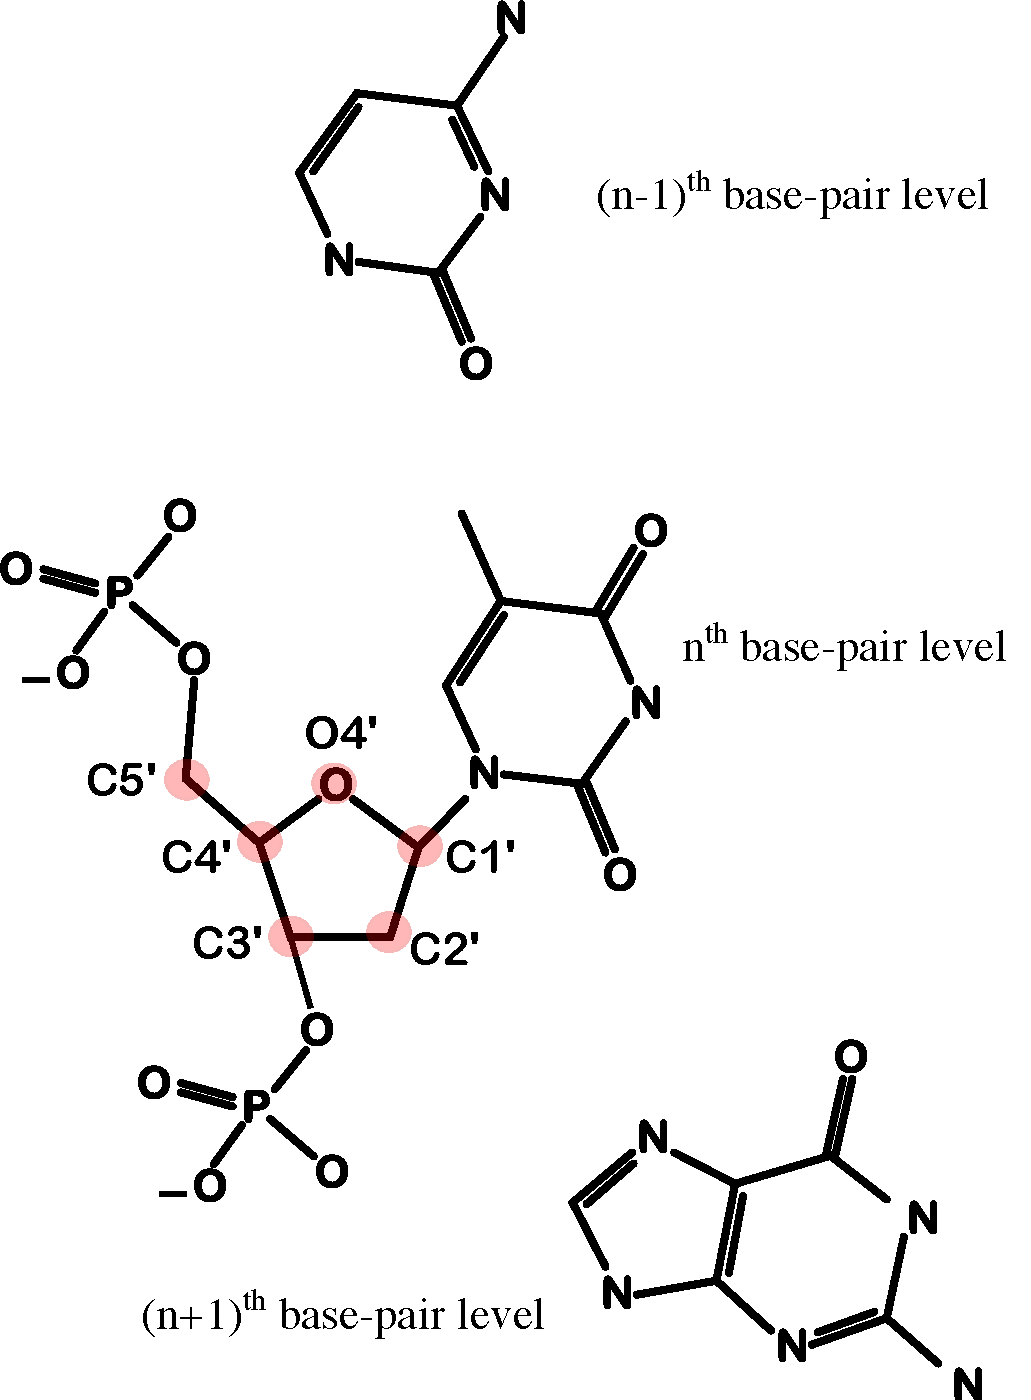
\includegraphics[scale=0.35]{images/DNA_chemical_structure_orig_2.pdf}
	\caption{A schematic diagram of a DNA strand with bases and phosphates (which can be obtained from the cgNA$+$ model) along with the missing sugar atoms highlighted in light red color. 
	The figure only focuses on one middle sugar ring; the rest of the sugar rings and the complementary strand are not shown.
	}
\label{c7:fig_backbone}
\end{center}
\end{figure}
\clearpage

\begin{figure}[t]
	\centering
	\begin{tikzpicture}[shorten >=1pt]
		\tikzstyle{unit}=[draw,shape=circle,minimum size=1.15cm]
		%\tikzstyle{hidden}=[draw,shape=circle,fill=black!25,minimum size=1.15cm]
		\tikzstyle{hidden}=[draw,shape=circle,minimum size=1.15cm]
 
		\node[unit](x0) at (0,3.5){$x_1$};
		\node[unit](x1) at (0,2){$x_2$};
		\node at (0,1){\vdots};
		\node[unit](xd) at (0,0){$x_D$};
 
		\node[hidden](h10) at (3,4){$y_1^{(1)}$};
		\node[hidden](h11) at (3,2.5){$y_2^{(1)}$};
		\node at (3,1.1){\vdots};
		\node[hidden](h1m) at (3,-0.5){$y_m^{(1)}$};
 
		\node(h22) at (5,0){};
		\node(h21) at (5,2){};
		\node(h20) at (5,4){};
		
		\node(d3) at (6,0){$\ldots$};
		\node(d2) at (6,2){$\ldots$};
		\node(d1) at (6,4){$\ldots$};
 
		\node(hN12) at (7,0){};
		\node(hN11) at (7,2){};
		\node(hN10) at (7,4){};
		
		\node[hidden](hN0) at (9,4){$y_1^{(H)}$};
		\node[hidden](hN1) at (9,2.5){$y_2^{(H)}$};
		\node at (9,1.1){\vdots};
		\node[hidden](hNm) at (9,-0.5){$y_m^{(H)}$};
 
		\node[unit](y1) at (12,3.5){$y_1$};
		\node[unit](y2) at (12,2){$y_2$};
		\node at (12,1){\vdots};	
		\node[unit](yc) at (12,0){$y_C$};
 		\draw[->] (x0) -- (h10);
		\draw[->] (x0) -- (h11);
		\draw[->] (x0) -- (h1m);
 		\draw[->] (x1) -- (h10);
		\draw[->] (x1) -- (h11);
		\draw[->] (x1) -- (h1m);
%%%%%%%%%%%%%%%%
		\draw[->] (xd) -- (h10);
 		\draw[->] (xd) -- (h11);
		\draw[->] (xd) -- (h1m);
		\draw[->] (hN0) -- (y1);
		\draw[->] (hN0) -- (y2);
		\draw[->] (hN0) -- (yc);
		\draw[->] (hN1) -- (y1);
		\draw[->] (hN1) -- (y2);
		\draw[->] (hN1) -- (yc);
%%%%%%%%%%%%%%%%
		\draw[->] (hNm) -- (y1);
		\draw[->] (hNm) -- (y2);
		\draw[->] (hNm) -- (yc);
        \draw[->,path fading=east] (h10) -- (h20);
		\draw[->,path fading=east] (h10) -- (h21);
		\draw[->,path fading=east] (h10) -- (h22);
        \draw[->,path fading=east] (h11) -- (h20);
		\draw[->,path fading=east] (h11) -- (h21);
		\draw[->,path fading=east] (h11) -- (h22);
		\draw[->,path fading=east] (h1m) -- (h20);
		\draw[->,path fading=east] (h1m) -- (h21);
		\draw[->,path fading=east] (h1m) -- (h22);
%%%%%%%%%%%%%%%%
		\draw[->,path fading=west] (hN10) -- (hN0);
		\draw[->,path fading=west] (hN11) -- (hN0);
		\draw[->,path fading=west] (hN12) -- (hN0);
		\draw[->,path fading=west] (hN10) -- (hN1);
		\draw[->,path fading=west] (hN11) -- (hN1);
		\draw[->,path fading=west] (hN12) -- (hN1);
		\draw[->,path fading=west] (hN10) -- (hNm);
		\draw[->,path fading=west] (hN11) -- (hNm);
		\draw[->,path fading=west] (hN12) -- (hNm);
		
		\draw [decorate,decoration={brace,amplitude=10pt},xshift=-4pt,yshift=0pt] (-0.5,4) -- (0.75,4) node [black,midway,yshift=+0.6cm]{input layer};
		\draw [decorate,decoration={brace,amplitude=10pt},xshift=-4pt,yshift=0pt] (2.5,4.5) -- (3.75,4.5) node [black,midway,yshift=+0.6cm]{$1^{\text{st}}$ hidden layer};
		\draw [decorate,decoration={brace,amplitude=10pt},xshift=-4pt,yshift=0pt] (8.5,4.5) -- (9.75,4.5) node [black,midway,yshift=+0.6cm]{$H^{\text{th}}$ hidden layer};
		\draw [decorate,decoration={brace,amplitude=10pt},xshift=-4pt,yshift=0pt] (11.5,4.15) -- (12.75,4.15) node [black,midway,yshift=+0.6cm]{output layer};
	\end{tikzpicture}
	\caption{Typical schematic diagram for a feed-forward Neural Network with $D$ input units, $C$ output units, and $H$ hidden layers each containing $m$ neurons.
	The input and output layers are considered as $0^\text{th}$ and $(H+1)^\text{th}$ layers. 
	}
	\label{c7:NN}
\end{figure}
\subsection{Feed-forward Neural Network}\label{c7:s1sb3}
Feed-forward Neural Networks (NNs), also known as multilayer perceptrons, are an important class of machine learning algorithms whose structure and name are inspired by neurons in the human brain. 
The goal of an NN is to approximate the true underlying function ($f^*$) for the given input ($X$) and output ($Y^*$) as $Y = f(X; \Theta)$ by learning the NN parameters $\Theta$. 
A typical NN diagram is shown in \cref{c7:NN}
with the zeroth layer as input layer (containing $D$ input units), $H$ hidden layers (containing $m$ neurons each), and the final layer as output layer (containing $C$ outputs). 
The inputs $X(x_1, x_2, ...  , x_D)$ can also be denoted as $(y_1^{(0)}, y_2^{(0)}, ...  , y_D^{(0)})$ and similarly, the outputs $Y(y_1, y_2, ... , y_C)$ as $(y_1^{(H+1)}, y_2^{(H+1)}, ... \ , y_C^{(H+1)})$.
$y_j^{(h)}$ is the output of the $j^\text{th}$ neuron in layer $h$ that is given as a function of the output of neurons in layer $h-1$ as,
\begin{equation}
y_j^{(h)} = f^{(h)}(y^{(h-1)}) = \Phi\left( \sum_{i}w_{i,j}^{(h)}y_i^{(h-1)} + b_j^{(h)}    \right) 
\label{c7:eq_neuron}
\end{equation}
where $i$ denotes the index of neuron in $(h-1)^\text{th}$ layer, $w_{i,j}^{(h)}$ is an NN parameter called weight that connects $i^\text{th}$ neuron in $(h-1)^\text{th}$ layer in $j^\text{th}$ neuron of the $h^\text{th}$ layer 
and $b_j^{(h)}$ is the bias term at $h^\text{th}$ layer for the $j^\text{th}$ neuron. 
Lastly, $\Phi(\cdot)$ is the activation function, which is often non-linear.  
Popular choices for  $\Phi(\cdot)$ include sigmoid function, inverse tangent function, and rectified linear unit (ReLU).
The final output, Y, is given as the composition of functions applied at every layer as
\begin{equation}
Y = f(X) = f^{(H+1)} \ \text{o} \ \cdot \cdot \cdot \ \text{o} \ f^{(2)} \ \text{o} \ f^{(1)}(X).
\label{c7:eq_out_NN}
\end{equation}
This step is also known as the forward pass. 

Given the training data with $P$ samples, $S_{Train} = {(X_p,Y^*_p)}_{p=1 \cdot \cdot P}$, the training of NN involves finding NN parameters, $w \and b$, such that it minimizes the cost function defined as 
\begin{equation}
\mathcal{L} = \frac{1}{P} \sum_{p=1}^{P}\left(Y^*_p - Y_p \right)^2.
\label{c7:eq_cost}
\end{equation}
The above loss function is the most popular choice called mean square error. 
Other popular choices include the mean absolute error, a combination of mean square error and mean absolute error, or some custom choices.
The NN training step is called the back-propagation step, and there exist several algorithms to minimize the loss function and, thus, optimize w and b starting from some random initialization.
Popular algorithms for the back-propagation step are gradient descent, stochastic gradient descent, and Adam optimizer. 

Before training NN, one must make various choices, including the number of hidden layers ($H$), neurons in each layer ($m$), activation function ($\Phi(\cdot)$), optimizer, network initialization, and loss function.
These choices are collectively called hyperparameters, and various options should be explored to find optimal hyperparameters for the given training data.
One of the standard techniques for searching in hyperparameter space is the k-fold cross-validation (CV) technique\cite{goodfellow2016deep}.
In the CV technique, a subset of training data is separated (randomly chosen), termed the validation set, used to test the performance of the NN trained on the remaining training data. 
This performance of the NN for a given choice of hyperparameters is called validation accuracy. 
The k-fold CV repeats the train-validation split k times so that all the samples in the training data become part of the validation data exactly once.
The most common choice for k is 5, i.e., in every split, $20 \%$ of the data are taken as validation data, and the model is trained on the remaining $80 \%$. 
Thus, using k-fold CV, one can compute the average validation accuracy for a given choice of hyperparameters, and based on this average validation accuracy, one can choose the optimal hyperparameters while searching in hyperparameter space. 

\subsection{Training data}
As described in \cref{c3}, we have performed 10 $\mu$s long MD simulations for 16 palindromic sequences (of length 24 bps) referred to as the training sequences in \Lbdna \ (see \cref{palinold}) to train the $\Pc_\text{DNA}$ in cgNA$+$ model.
To train the NN, we have used snapshots from the same training data.
Note that the training sequences in \Lbdna \ contain all possible trimers with almost the same frequency.
We have used the following steps to obtain the training data for NN:
\begin{itemize}
\item[i)] In the MD time-series of each training sequence, we sub-sampled snapshots such that the configurations are uncorrelated (100 picoseconds apart from each other). It leads to $16\cdot10^5$ snapshots in the training data, since we have $10 \mu$s of MD simulations for 16 sequences. Subsequently, we removed snapshots with broken H-bond (as done in training the cgNA$+$ model), which discarded $\approx 15 \%$ of the initial training data; thus, $0.85 \cdot 16\cdot10^5$ snapshots.
\item[ii)] Each MD configuration is split into trimers centered around the middle sugar ring, as shown in \cref{c7:fig_backbone} while reading separately from both strands. 
It led to 22 trimers per strand for each configuration (as sugar rings associated with terminal base-pairs are ignored).
Thus, the total samples to train NN $\approx 0.85 \cdot 16 \cdot 10^5 \cdot 2 \cdot \ 22$ where the atomistic coordinates of the phosphates and bases are inputs, while the sugar atoms are outputs.
\item[iii)] Before training, we have aligned all the trimers about its central base, i.e., the frame associated with the central base is taken as $\{I,\v 0\}$ where $I \in \R^{3\times3}$ is an identity matrix and $\v 0 \in R^{3\times1}$ is a zero vector. 
\end{itemize} \clearpage


\begin{table}
\begin{center}
\begin{small}
\begin{tabular}{c c c c c c c c c }
\hline
Model & Weight  & Optimizer  & Batch  & Epoch & Activation  & Number   &  Hidden & Learning  \\
& initialization & &  size &  &  function & of nodes  &  layers & rate \\
 \hline
 \hline 
\vspace{-0.2cm}
\multicolumn{9}{c}{} \\ 
\multicolumn{9}{c}{\textbf{(a) Hyperparameter space explored}} \\ 
\vspace{-0.2cm}
\multicolumn{9}{c}{} \\  
& Xavier normal  & Adam    & 32   & 50  & ReLU    & 200 to 1800 &  2, 4,  & 0.001   \\
& Random normal  & SGD     & 64  & 100 & tanh    & in steps of 200 & 6, 8  & 0.005   \\
&  &  & 128 & 200 & sigmoid & &  & \\
\hline
\hline
\vspace{-0.2cm}
\multicolumn{9}{c}{} \\  
\multicolumn{9}{c}{\textbf{(b) Optimal hyperparameters}} \\
\vspace{-0.2cm}
\multicolumn{9}{c}{} \\ 
RRR & Xavier normal  & Adam    & 32   & 200  & ReLU    & 1200 &  4  & 0.001 \\
RRY & Xavier normal  & Adam    & 32   & 200  & ReLU    & 1200 &  4  & 0.001 \\
RYR & Xavier normal  & Adam    & 32   & 200  & ReLU    & 1800 &  4  & 0.001 \\
YRR & Xavier normal  & Adam    & 32   & 200  & ReLU    & 1200 &  4  & 0.001 \\
YYR & Xavier normal  & Adam    & 32   & 200  & ReLU    & 1200 &  4  & 0.001 \\
YRY & Xavier normal  & Adam & 32   & 200  & sigmoid    & 400 &  4  & 0.0005 \\
RYY & Xavier normal  & Adam    & 32   & 200  & ReLU    & 1800 &  6  & 0.001 \\
YYY & Xavier normal  & Adam    & 32   & 200  & ReLU    & 400 &  4 & 0.0005 \\
\end{tabular}
\end{small}
\end{center}
\caption{(a) Hyperparameters space explored and (b) the optimal hyperparameters found for neural networks trained for each trimer.}
\label{c7:tab_hyper}
\end{table}

Since the overarching aim of this work is to fit the sugar ring in cgNA$+$ predicted coarse-grained configurations, which have rigid phosphates and rigid bases, i.e., fixed position of atoms within a given rigid body.
Therefore, the model should also be trained on similar data rather than crude MD snapshots, which have non-rigid phosphates and bases.
Thus, the input data for the NN are the best-fit ideal coordinates in the phosphate and base units, which are obtained by first fitting the frames in the MD snapshots (refer \cref{c2:sec1}) and then re-embed ideal atoms as described in \cref{c7:eq_T_I_C}. 

\subsection{Implementation}
In the previous sections, we have described the typical architecture of the NN and the training data.
In this section, we have discussed the implementation of the NN to predict the location of sugar atoms from the positions of neighboring bases and phosphates.
In other words, we have trained the NN for which the input is the atomic positions of the three nearest bases and the two nearest phosphates to the sugar ring on the same strand, and the output is the coordinate of the sugar atoms.  It is mathematically described in \cref{c7:eq_NN_function}.

One of the crucial aspects of the NN architecture pertinent to this implementation is that the NN has a fixed number of input features (once chosen).
However, the number of atoms in the neighboring bases depends on the type of base (A/T/C/G). 
A/G are purines with more atoms, while C/T are pyrimidines with fewer atoms.
Therefore, we have trained eight different NNs for eight possible trimers in the pyrimidine and purine alphabets.

\clearpage
\begin{figure}[H]
	\begin{center}
	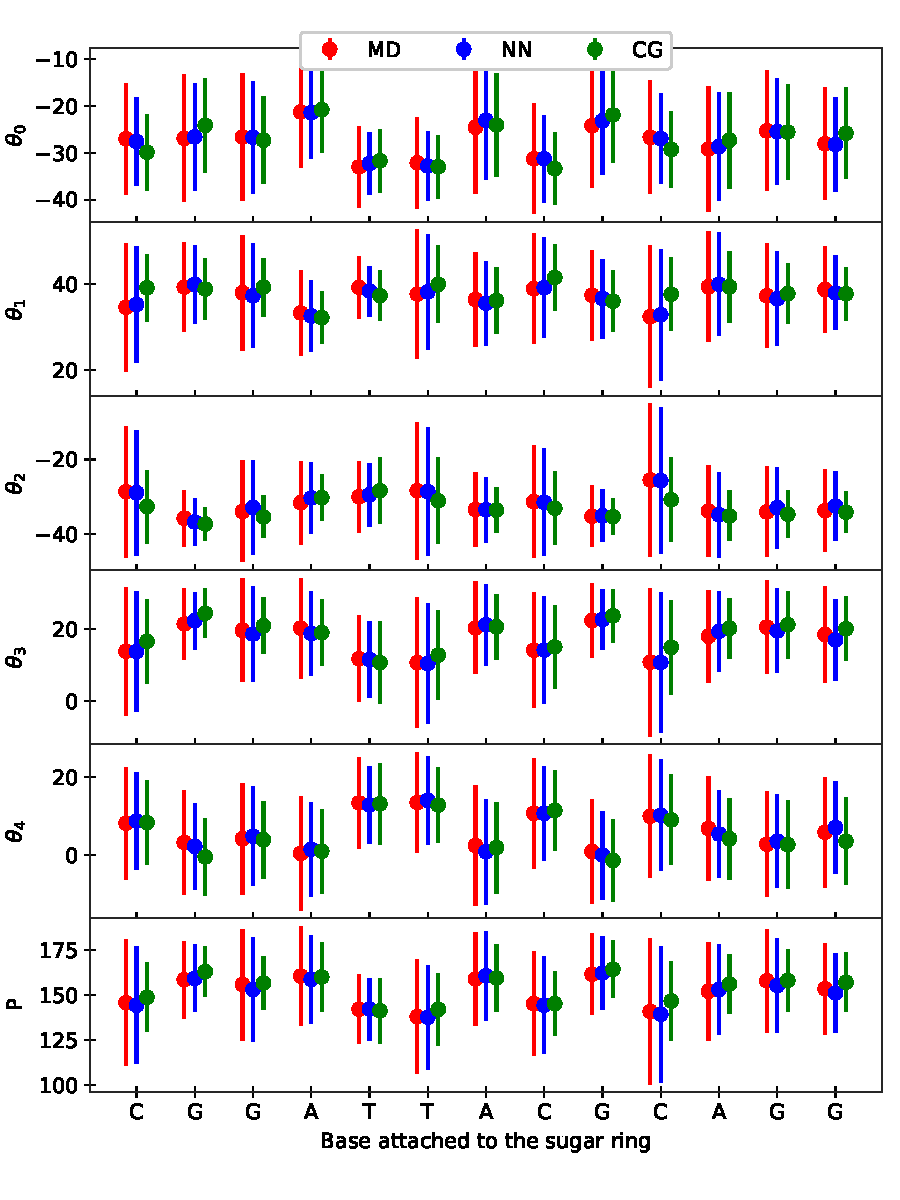
\includegraphics[width=15cm]{images/puck_stats_20_1.pdf}
	\caption{Sugar pucker angles on Watson strand of sequence index 20 in \Lbdna \ (GCGGATTACGCAGGC). 
    The parameters observed in MD simulations (labeled as MD) are in red, obtained by re-fitting sugar in coarse-grained MD snapshots (labeled as NN) are in blue, and obtained by fitting sugar in an ensemble of coarse-grained configurations generated by the cgNA$+$ Monte Carlo (labeled as CG) are in green.
    The ensemble mean and standard deviation for a given parameter are plotted as $\bullet$ and vertical line, respectively.}
\label{c7:fig3}
\end{center}
\end{figure}

\begin{figure}[H]
	\begin{center}
	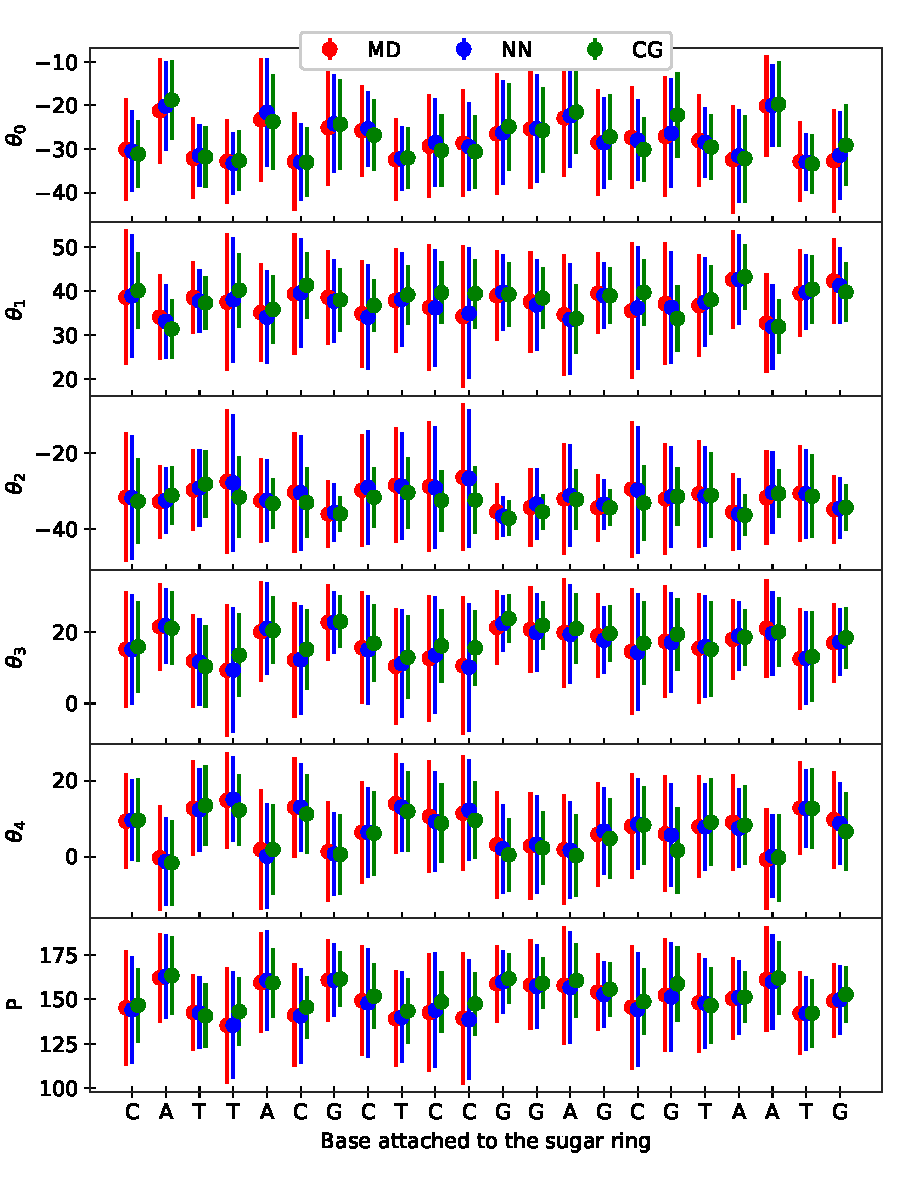
\includegraphics[width=15cm]{images/puck_stats_17_1.pdf}
	\caption{Sugar pucker angles on Watson strand of sequence index 17 in \Lbdna \ (GCATTACGCTCCGGAGCGTAATGC). 
    The parameters observed in MD simulations (labeled as MD) are in red, obtained by fitting sugar in coarse-grained MD snapshots (labeled as NN) are in blue, and obtained by fitting sugar in an ensemble of coarse-grained configurations generated by the cgNA$+$ Monte Carlo (labeled as CG) are in green. 
    The ensemble mean and standard deviation for a given parameter are plotted as $\bullet$ and vertical line, respectively.}
\label{c7:fig4}
\end{center}
\end{figure}

\subsubsection{Hyperparameters selection}
Before training the final (best-fit) NN model, one must choose the hyperparameters for NN. 
We have chosen the hyperparameters for each NN based on the average validation accuracy as described in \cref{c7:s1sb3}.
We have used a five-fold CV, i.e., randomly split the total training data (for each trimer) into five equal sets, of which four sets were used as training data, while the remaining one was used as validation data.
This process is repeated five times such that each set becomes the validation data exactly once.
Based on this average validation accuracy, we have selected the hyperparameters for the best-fit model.
In \cref{c7:tab_hyper}, we have listed the hyperparameter space explored to find the optimal choice for the best-fit model.
In total, we have explored $7,776$ combinations, of which many choices gave a comparable average validation accuracy.
Finally, for each trimer model, the set of hyperparameters with the highest average validation accuracy was selected as the optimal hyperparameters as tabulated in \cref{c7:tab_hyper}.
In particular, we found that the Adam optimizer performed best with 200 epochs (the number of times the training data pass through the algorithm), batch-size (number of samples in one iteration of training) of 32, and Xavier normal initialization of the neural network parameters.
The ReLU activation function generally works best, and the optimal choices for the number of neurons and hidden layers are different for different trimer models. 

\subsubsection{Best-fit model} 
%\rs{more details on the computer archi ... This point raises also the question of software that was created during the project, how it is accessible and how it will be curated (if at all). I could not find any information on codes, code listing, link to a repository, etc.}
Once the optimal hyperparameters are found (listed in \cref{c7:tab_hyper}), the best-fit model is trained for each trimer using the complete training data.
The training of each model took approximately 12 hours on one CPU. 


\subsection{How accurate is the model?}
In this section, we have discussed the NN accuracy in predicting sugar atom coordinates. 
First, we have described the test data and then quantified NN performance.

\subsubsection{Test data for model}
Test data should not be involved in model training or hyperparameter selection.
Recall that NNs are trained on MD snapshots that are 100 picoseconds apart in the MD times-series (which has snapshots at two picosecond intervals) of the training sequences in \Lbdna.
Therefore, in principle, the remaining MD snapshots not used in NN training can be used as test data.
A more severe test would be to check the model prediction accuracy for sequences not used in the training data, i.e., test sequences in \Lbdna.
In the following section, we have compared the predictions with observations in MD simulations for two sequences that are not part of the training library. 

\subsubsection{Model accuracy in the prediction of sugar atoms position}
The cgNA$+$ sugar module predicts the location of sugar atoms in any cgNA$+$ coarse-grained configuration.
Then, various dihedral angles (commonly used to characterize the DNA backbone and sugar ring) can be computed from these atomic positions.
We have assessed the quality of the model predictions for a) atomistic coordinates of sugar and b) various backbone dihedrals and sugar pucker angles for two test sequences (indices 17 and 20 in \Lbdna).

To evaluate the accuracy of the cgNA$+$ sugar module, we first have coarse-grained MD snapshots (by fitting phosphate and base frames) and then fine-grain those coarse-grained snapshots using the cgNA$+$ sugar module.
The mean square error per degree of freedom (dof) in predicting the location of sugar atoms for the test data is approximately 0.005 \AA$^2$ or $\approx 0.07$ \AA \ as the root mean square error per dof.
The statistics are obtained from $10^5$ snapshots (minus snapshots with broken H bond) for each of two test sequences (indices 17 and 20 in \Lbdna).
Thus, in absolute terms, the mean error in the predictions of the cgNA$+$ sugar module for test sequences is negligible.
Compared to the reconstruction error in the cgNA$+$ model, which is $\approx$ 0.003 \AA$^2$ or (rad/5)$^2$ per dof in terms of the Mahalanobis distance (see \cref{c4:tab1_errors} for more details), the prediction error in the cgNA$+$ sugar module is only slightly larger.
It highlights that the cgNA$+$ sugar module can accurately fine-grain any cgNA$+$ coarse-grained configuration.

The standard parameters for analyzing the DNA backbone and sugar conformations are dihedral angles.
In \cref{c7:fig3,c7:fig4}, we have plotted the sugar ring dihedral angles and the pseudo-rotation phase angle (\textbf{\textsc{P}}) (defined in \cref{c1:s2:sb1}) for two test sequences with MD observations in red and the corresponding NN predictions (for the same MD configurations) in blue.
The following observations can be made from the figures:
\begin{itemize}
\item Both the mean and standard deviation for various parameters are highly sequence-dependent.
\item NNs capture the distribution of various parameters exceptionally well, with mean values almost identical and standard deviation slightly smaller in the predictions.
\item In a one-to-one comparison of the configurations in the ensemble, the Pearson correlation for any parameter is greater than 0.9.
\end{itemize}

Furthermore, in \cref{c7:fig5,c7:fig6}, we have plotted various backbone dihedral angles (defined in \cref{c1:s2:sb1}). 
First, note that the sugar pucker angles are defined using the sugar atoms predicted by the NNs; in contrast, backbone dihedral angles involve some atoms that are part of either rigid base or rigid phosphate.
For instance, $\alpha_n$ is defined as the dihedral angle between O3$^\prime_{n-1}$--P$_{n}$--O5$^\prime_{n}$--C5$^\prime_{n}$ (see \cref{c1:fig3}) involving frozen atoms O3$^\prime_{n-1}$, P$_{n}$, and O5$^\prime_{n}$.
Therefore, a larger prediction error can be expected in the backbone dihedral angles because of the rigid base/phosphate assumption, which can not be attributed to the NNs performance.
As can be observed in \cref{c7:fig5,c7:fig6}, NNs capture the dihedral angles of the backbone; their mean and standard deviation are almost similar and highly dependent on the underlying sequence.
However, one can also notice that the various backbone dihedrals are consistently underestimated or overestimated (only a few degrees) irrespective of the sequence, e.g., $\alpha$ and $\zeta$ are overestimated, while the rest are underestimated.
Lastly, in \cref{c7:fig7}, we have compared the backbone conformations in the two test sequences by plotting \% B\rom{2} population identified as $\epsilon - \zeta > 0$. 
NNs predictions systematically overestimate \% B\rom{2} conformations compared to those observed in the corresponding MD simulations, which can be expected as a slight underestimation and overestimation of $\epsilon$ and $\zeta$, respectively, have a pronounced effect on \% B\rom{2} or B\rom{1} conformations.

\begin{figure}[H]
	\begin{center}
	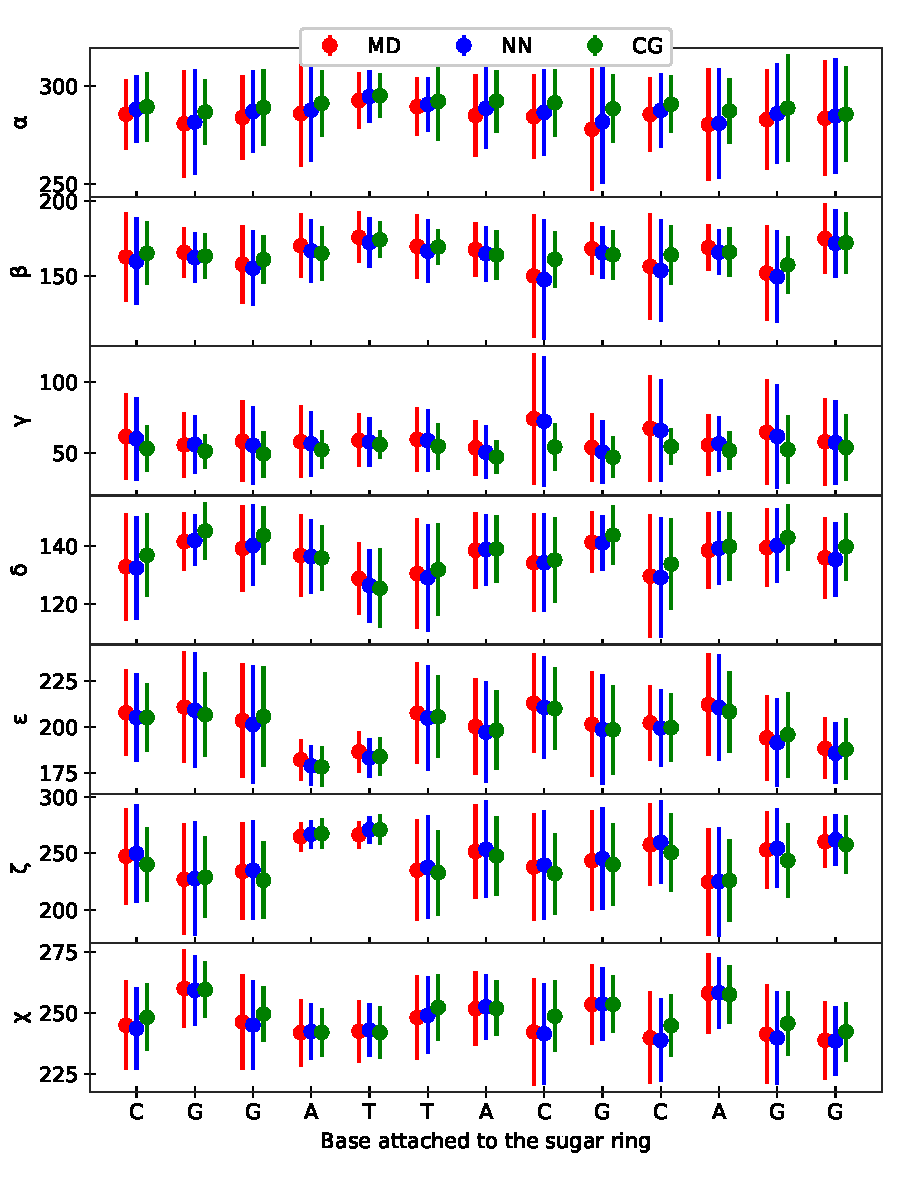
\includegraphics[width=15cm]{images/dihed_stats_20_1.pdf}
	\caption{Backbone dihedrals (on the Watson strand) for sequence index 20 in \Lbdna \ (GCGGATTACGCAGGC). The parameters observed in MD simulations (labeled as MD) are in red, obtained by fitting sugar in coarse-grained MD snapshots (labeled as NN) are in blue, and obtained by fitting sugar in an ensemble of coarse-grained configurations generated by the cgNA$+$ Monte Carlo (labeled as CG) are in green. 
    The ensemble mean and standard deviation for a given parameter are plotted as $\bullet$ and vertical line, respectively.
	}
\label{c7:fig5}
\end{center}
\end{figure}

\begin{figure}[H]
	\begin{center}
	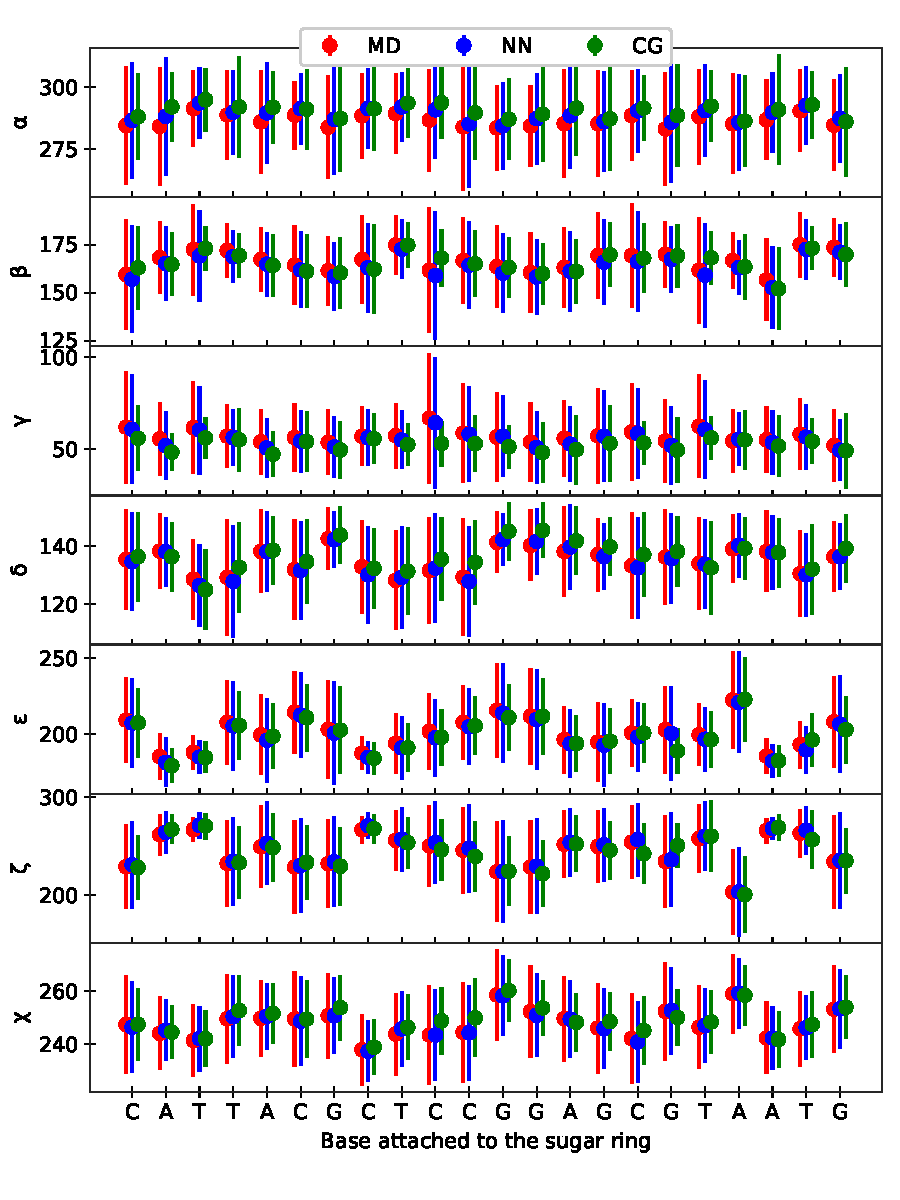
\includegraphics[width=15cm]{images/dihed_stats_17_1.pdf}
	\caption{Backbone dihedrals (on the Watson strand) for sequence index 17 in \Lbdna \ (GCATTACGCTCCGGAGCGTAATGC).  
    The parameters observed in MD simulations (labeled as MD) are in red, obtained by fitting sugar in coarse-grained MD snapshots (labeled as NN) are in blue, and obtained by fitting sugar in an ensemble of coarse-grained configurations generated by the cgNA$+$ Monte Carlo (labeled as CG) are in green. 
    The ensemble mean and standard deviation for a given parameter are plotted as $\bullet$ and vertical line, respectively.
	}
\label{c7:fig6}
\end{center}
\end{figure}

\begin{figure}[H]
  \begin{subfigure}{15cm}
    \centering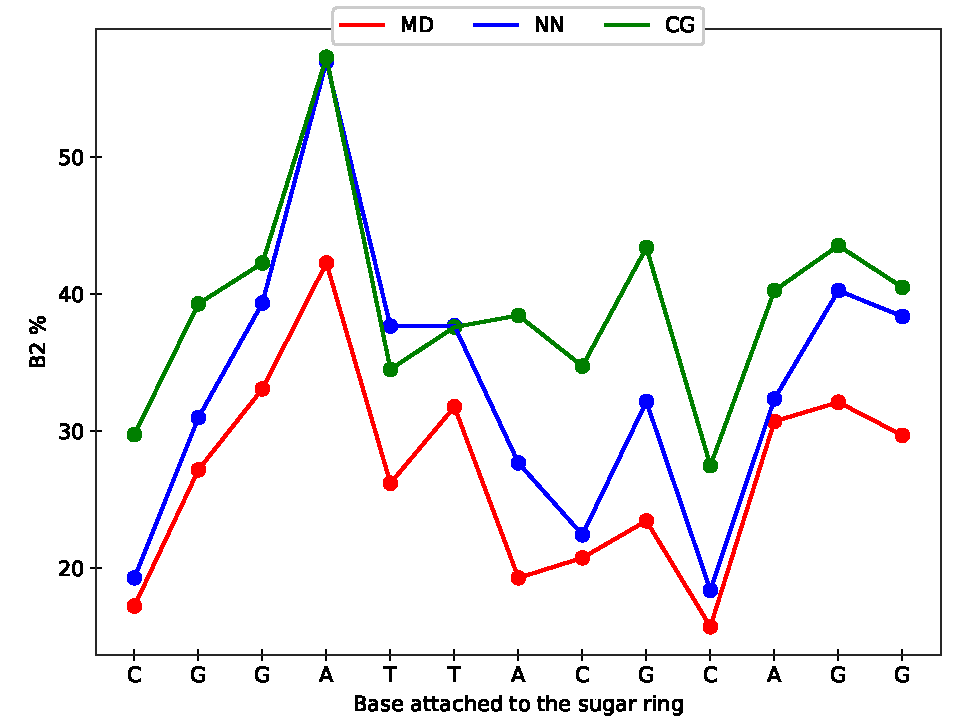
\includegraphics[scale=0.8]{images/B1_B2_dihed_stats_20_1.pdf}
    \centering\caption{B\rom{2} \% on the Watson strand for sequence index 20 in \Lbdna \ (GCGGATTACGCAGGC)}
  \end{subfigure} 

  \begin{subfigure}{15cm}
    \centering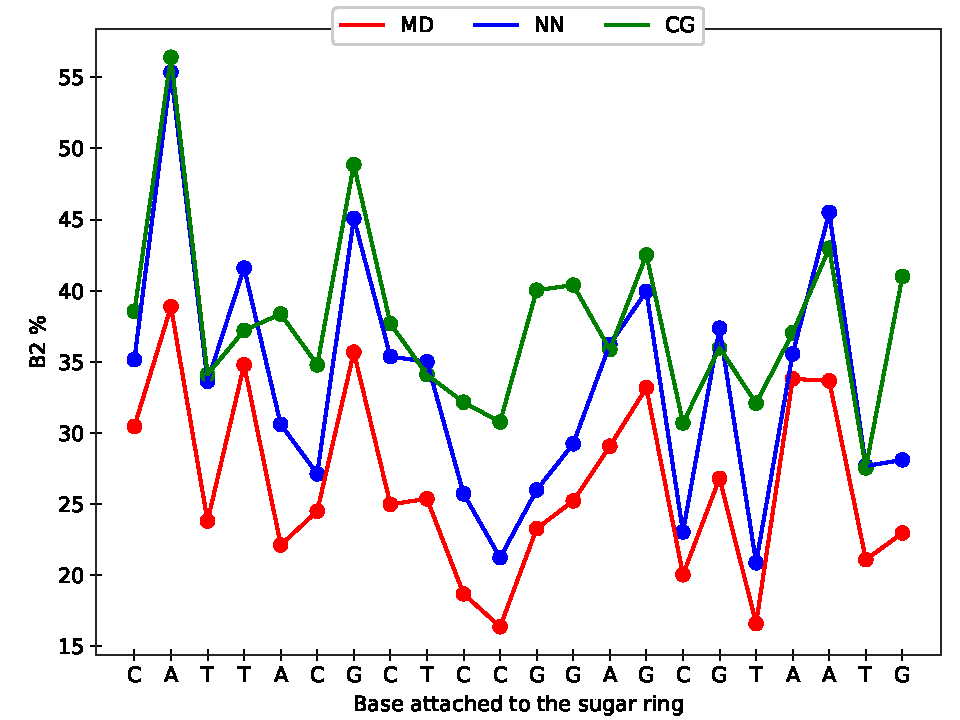
\includegraphics[scale=0.8]{images/B1_B2_dihed_stats_17_1.pdf}
    \centering\caption{B\rom{2} \% on the Watson strand for sequence index 17 in \Lbdna \ (GCATTACGCTCCGGAGCGTAATGC)}
  \end{subfigure}
\centering\caption{
B\rom{2} \% on the Watson strand for sequence indices 20 and 17 in \Lbdna. 
    The parameters observed in MD simulations (labeled as MD) are in red, obtained by fitting sugar in coarse-grained MD snapshots (labeled as NN) are in blue, and obtained by fitting sugar in an ensemble of coarse-grained configurations generated by the cgNA$+$ Monte Carlo (labeled as CG) are in green. 
    The ensemble mean and standard deviation for a given parameter are plotted as $\bullet$ and vertical line, respectively.
}
\label{c7:fig7}
\end{figure}


\section{Applications of the cgNA$+$ sugar module}
The primary goal of the cgNA$+$ sugar module is to fine-grain any cgNA$+$ coarse-grained configuration.
It allows to predict a complete atomistic equilibrium structure for an arbitrary sequence.
Moreover, using the cgNA$+$ Monte Carlo code (refer \cref{c2:sec6}), one can obtain an ensemble of configurations (in cgNA$+$ coarse-grained coordinates) and then using the cgNA$+$ sugar module, an ensemble of atomistic configurations.
This ensemble allows for studying backbone and sugar-pucker conformations for any sequence.
In particular, we have predicted the ensemble of atomistic configurations (using the cgNA$+$ Monte Carlo code and sugar module) for sequence indices 17 and 20 (of \Lbdna \ listed in \cref{palinold}) and plotted the various pucker angles, dihedral angles and backbone conformations in \cref{c7:fig3,c7:fig4,c7:fig5,c7:fig6,c7:fig7} in green.
For the sugar pucker angles shown in \cref{c7:fig3,c7:fig4}, the two data sets, a) MD observations and b) ensemble of atomistic configurations obtained using the cgNA$+$ Monte Carlo code, are close in terms of mean and standard deviation (standard deviation is greater in MD observations).
However, there are some noticeable exceptions, for example, C at the 11$^\text{th}$ position of index 20 as shown in \cref{c7:fig3}.
Similar observations can also be made for the dihedral angles and conformations of the backbone in \cref{c7:fig5,c7:fig6,c7:fig7}.
We would like to highlight that the provided MD statistics are for 10 $\mu$s of simulation data which took approximately two months (for a sequence of length 24 base-pairs) on a highly efficient GPU node (containing 2 Xeon-Gold processors and 2 NVIDIA V100 PCIe 32 GB GPUs); in contrast, the ensemble of $10^5$ atomistic configurations obtained using the cgNA$+$ tools merely took an hour.
Thus, this approach provided an accurate and highly efficient alternative to obtain a sampling of configurations for any sequence.
Such an analysis can be easily performed for a large number of sequences.
It will be beneficial to generate such an ensemble for some mechanically exceptional sequences discovered using the cgNA$+$ model, for instance, sequences with extreme groove widths or persistence lengths, as discussed in \cref{c4}.
This analysis is not performed in this thesis, as the authors believe that there is scope for improvement in the current cgNA$+$ sugar module, as discussed in the next section; therefore, an extensive analysis of interesting sequences will be undertaken in the future.

Another application of this module is to obtain a sequence-dependent atomistic equilibrium structure for an arbitrary sequence, which can then be used as a starting point for the MD simulations. 
Note that the starting structure in an MD simulation is crucial and desirable that it is close to the equilibrium structure under the given physical conditions.
A starting structure far from the equilibrium structure may take a prohibitively long simulation time to equilibrate.
There are several reliable sources to obtain an initial structure for short linear NA fragments, such as the nucleic acid builder (NAB) in AMBERTOOLS 18~\cite{amber}.
However, for large systems, in particular, dsDNA mini-circles (typically are of length 60-500 base-pairs), obtaining a good initial structure is non-trivial and crucial as full atomistic MD simulation is computationally expensive.
Previous studies~\cite{lankavs2006kinking} have used JUMNA software~\cite{lavery1995jumna} to obtain the initial structures, and then the energy of that structure is minimized using some force fields.
%There also exists some other approaches to obtain the initial structures of the DNA mini-circles. 
In particular, Glowacki et al.~\cite{glowackithesis,beaud2021using} developed an algorithm to compute the equilibrium structure of the dsDNA mini-circle (in cgDNA/cgDNA$+$ internal coordinates) for a given sequence and linking number from a linear groundstate predicted by the cgDNA/cgDNA$+$ model.
This algorithm, combined with the cgNA$+$ sugar module, presents an excellent method to obtain a sequence-dependent equilibrium atomistic structure that can be used to start MD simulations.
Such an accurate sequence-dependent equilibrium structure for dsDNA mini-circles should take significantly less simulation time to equilibrate in MD simulations.
Note that the location of sugar atoms predicted by the cgNA$+$ sugar module for dsDNA mini-circles might not be highly accurate compared to linear fragments (as the NNs are trained on linear fragments data), in particular, for highly overwound or underwound dsDNA mini-circles, but it is still an excellent tool to obtain a good initial structure for dsDNA mini-circles.
At the time of the thesis writing, we do not have any MD simulation results for dsDNA mini-circles to compare the predicted dsDNA mini-circle equilibrium structure with the MD observations, but in the future, such a comparison will help validate and further improve the cgNA$+$ sugar module for dsDNA mini-circles.

\section{Limitations of the cgNA$+$ sugar module and  improvement directions}

We would like to emphasize that the current version of the module presented in this chapter has a further scope of improvement in several directions.
In particular, we have used only the feed-forward architecture of the NNs, which works reasonably well. 
However, other popularly used NN architectures, such as recurrent and long-short-term memory NN, might improve the predictions.

Calculating the dihedral angles and backbone conformational state involves phosphate or base atoms that are assumed to be frozen in the cgNA$+$ configurations.
This approximation for phosphate and base as rigid bodies is reasonable; however, it might lead to erroneous backbone dihedral angles.
In particular, the atoms within a phosphate group fluctuate more and are involved in the computation of most dihedral angles.
Therefore, a possible solution to improve the prediction of the backbone dihedral angles is to allow perturbations in the phosphate atoms.
This can be implemented by predicting perturbations in the phosphate atoms (or perturbed phosphate position) using the NNs as additional outputs.

Finally, in the current module, we do not have parameters for the terminal sugar as it does not have the same number of neighbors as the interior sugar.
It requires training new networks with a different number of input features.
Moreover, the current module is limited to dsDNA only, and it would be particularly beneficial to extend the module for dsDNA with epigenetic base modifications that significantly impact backbone conformation and sugar puckering modes~\cite{banyay2002structural,liebl2019methyl}.
The module should also be extended for dsRNA and DRH for completeness.